%!TEX root = ../thesis.tex

\chapter{Related Work}
\label{chapter_related_work}

While existing practices require tutorial authors to create instructions manually, HCI and Computer Graphics communities have introduced novel technologies for authoring tutorials, including automatic generation methods and interactive editing tools.
%
In this chapter, I survey state-of-the-art techniques for generating instructions for both software applications (Section \ref{related_software}) and physical tasks (Section \ref{related_physical}).
%
Furthermore, existing instructions are mainly offered in the forms of conventional media, such as static tutorials (print-outs or web) or videos. With software systems, \keyword{interactive tutorials} have been introduced for learners to interactively review instructional content. I will discuss various forms of such kind of instructions by prior research, which leads to a discussion on the remaining gaps in tool support for creating and navigating instructional content.
%
Finally, in Section \ref{related_videos}, I review the methods of video analysis and playback.

% -------------------------------------------

\section{Instructions for Software Applications}
\label{related_software}

\subsection{Input Event Visualization}

% real-time
Studies have shown that visualizing input events during user operations can provide better learnability of software applications~\cite{Dixon:2010fb}. Events can range from low-level, application agnostic input device events (e.g., mouse actions, cursor movements, or keyboard strokes) to higher level, application-dependent information (e.g., menu selections or UI component changes).
%
Commercial tools such as Mouseposé\footnote{\url{http://www.boinx.com/mousepose}} and ScreenFlow\footnote{\url{http://www.telestream.net/screenflow}} visualize mouse events and keystrokes with special effects, e.g., drawing a circle around a mouse cursor (see Figure~\ref{fig:related_realtime} top). These tools capture input information (e.g., mouse position and event type) and render visualization on top of the screen activities. This approach has been widely used by online video tutorial authors. However, it does not consider application context, which can be difficult for learners who want to follow specific instructions at a semantic level, such as observing a complete text field or drop-down menu option.
% Some further enable video editing techniques, including zooming in/out  and panning.

To visualization UI components (e.g., a checkbox, button, or editable text field), Dixon \ea{}'s Prefab~\cite{Dixon:2010fb,Dixon:2011:CHP:1978942.1979086} provides pixel-based enhancements in real-time by detecting target features, such as region corners. This semantic understanding of GUI elements enables component-based highlighting effects, such as afterglows~\cite{Baudisch:2006:PET:1166253.1166280} that visualize user operations (see Figure~\ref{fig:related_realtime} bottom left) and Bubble Cursor~\cite{Grossman:2005:BCE:1054972.1055012}, a target-aware pointing technique that suggests the nearest target (see Figure~\ref{fig:related_realtime} bottom right).

\begin{figure*}[t!]
  \centering
  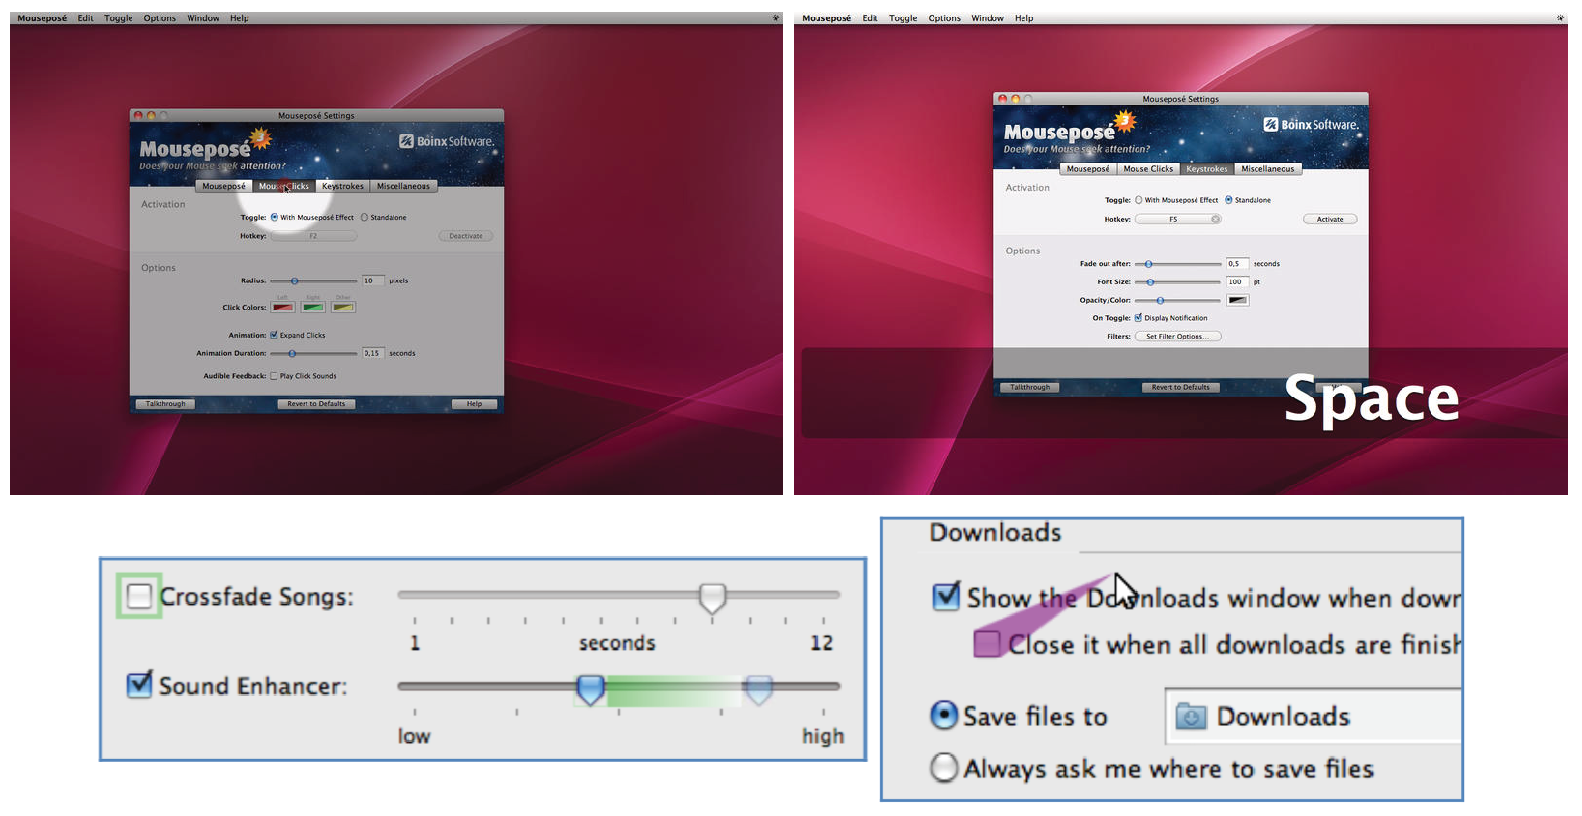
\includegraphics[width=0.7\textwidth]{\background/fig/realtime/realtime}
  \caption{Real-time visual enhancements on GUI applications: The top row shows how Mouseposé highlights a mouse cursor (left) and keyboard input (right); The bottom row presents Prefab~\cite{Dixon:2010fb}'s results of reverse engineering that identifies UI components and enables visualizations during author operations, such as afterglow~\cite{Baudisch:2006:PET:1166253.1166280} (left) and target-aware~\cite{Grossman:2005:BCE:1054972.1055012} (right) effects.}
  \label{fig:related_realtime}
\end{figure*}

\begin{figure*}[t!]
  \centering
  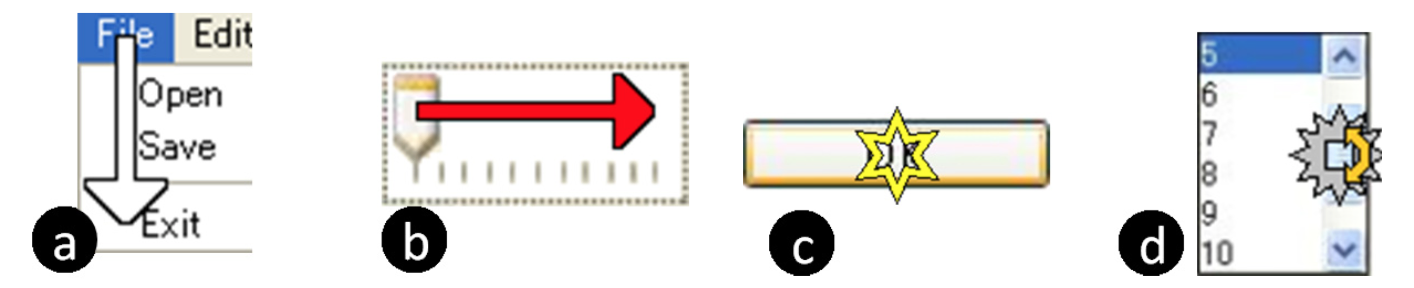
\includegraphics[width=0.6\textwidth]{\background/fig/software_viz/Nakamura_and_Igarashi}
  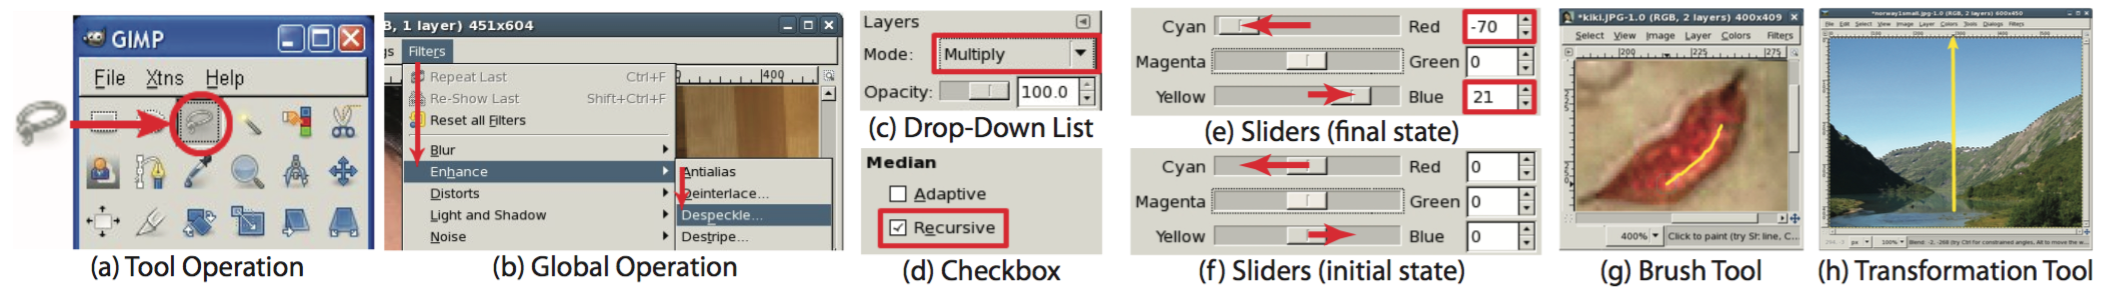
\includegraphics[width=\textwidth]{\background/fig/software_viz/Grabler}
  \caption{Example screenshots where mouse operations are automatically rendered, including (top) mouse move, drag, click, and wheel (a-d) by Nakamura and Igarashi~\cite{Nakamura:2008:ASV:1449715.1449721} and (bottom) application-specific operations (a-b), parameters (c-f), and manipulations (g-h) by Grabler \ea{}~\cite{Grabler:2009jj}.}
  \label{fig:related_events}
\end{figure*}

% in screenshots
The above methods enable real-time visualization of input events when operating an application, which are useful for following a video tutorial. However, they may not effectively present continuous actions, such as navigating a menu from the root to a sub-panel. For screenshot images in a static tutorial, visualizing input actions with motion arrows is a common technique to provide a sense of direction and start and end positions.
%
Researchers have investigated automatic approaches that capture and visualize these types of events in representative screenshots from author demonstrations. Nakamura and Igarashi~\cite{Nakamura:2008:ASV:1449715.1449721} proposed a capturing and rendering system independent to GUI applications. Their system logs mouse events of a software demo process, including mouse moving, dragging, and clicking. Operations are rendered as markers and arrows on screenshot images to present the linear event history (see Figure~\ref{fig:related_events} top).
%
Grabler \ea{}'s approach~\cite{Grabler:2009jj} further annotates a screenshot with bounding boxes and call-outs, which help learners identify parameters and options of software functionalities (see Figure~\ref{fig:related_events} bottom).

% summary
Our systems adopt some of these successful techniques to enhance visual instructions. By capturing event information at both input device and application levels, we visualize author operations based on different playback modes.
%
During \emph{video playback}, MixT shows mouse trails and actions, and DemoWiz overlays glyphs and arrows to guide viewers from the current input action to the next.
%
In a \emph{static}, step-by-step tutorial, MixT renders screenshot images with mouse visualizations, such as highlighting a drop-down menu.

% -------------------

\subsection{Workflow Capturing and Tutorials}
In addition to visualizing input events, it is important to present the entire workflow in a tutorial and provide concise instructions.
%
Grabler \ea{}'s system~\cite{Grabler:2009jj} generates a step-by-step tutorial from author demonstration (see Figure~\ref{fig:related_static}). Designed for instructing image manipulation tasks, it includes textual description from templates, such as \iquote{Select the \textbf{path tool} from the \textbf{toolbar} to \textbf{create and edit paths}.} The generated text and annotated images of operations are presented in a document to describe a workflow. Their work is available as a Photoshop plug-in\footnote{Adobe labs. Tutorial Builder. \url{http://labs.adobe.com/technologies/tutorialbuilder/}}.
% analyzes the application context, including facial features and outdoor scenes in manipulated images.
%
Such demonstration-based approaches have been applied to generate instructions for software that involves complicated manipulations or gestures, including 3D mesh construction~\cite{Denning:2011fy} and touch-based mobile applications~\cite{Wang:2014:EAC:2556288.2557407}.
%
Beyond logging input events during an author demonstration, researchers have shown that workflows and software content can be acquired using computer vision from analyzing desktop regions~\cite{Yeh:2009dh,Chang:2011vd} and existing screencast videos~\cite{Banovic:2012kd}.

\begin{figure*}[t!]
  \centering
  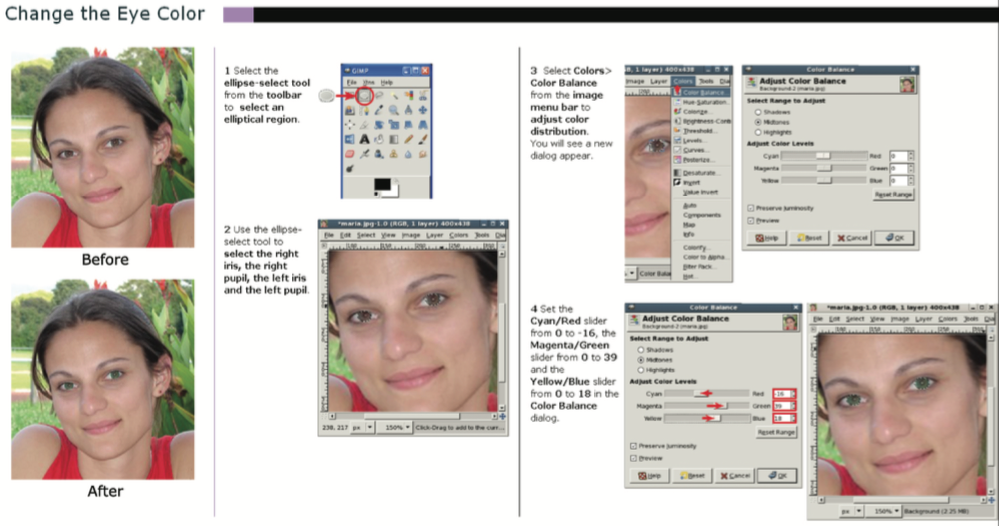
\includegraphics[width=0.8\textwidth]{\background/fig/related_static/grabler}
  \caption{Example static tutorial automatically generated by Grabler \ea{}'s system~\cite{Grabler:2009jj}.}
  \label{fig:related_static}
\end{figure*}

To compare effects of individual operations in a workflow, showing a list of ``before'' and ``after'' thumbnails, video clips, and event timeline can be effective \cite{Grossman:2010jz}, especially for image manipulation tasks (see Figure~\ref{fig:related_comparison} left).
%
When there are multiple workflows that create similar results, a union graph and side-by-side documents are useful for comparing operations~\cite{Kong:2012:DTR:2207676.2208549} (see Figure~\ref{fig:related_comparison} right).

\begin{figure*}[t!]
  \centering
  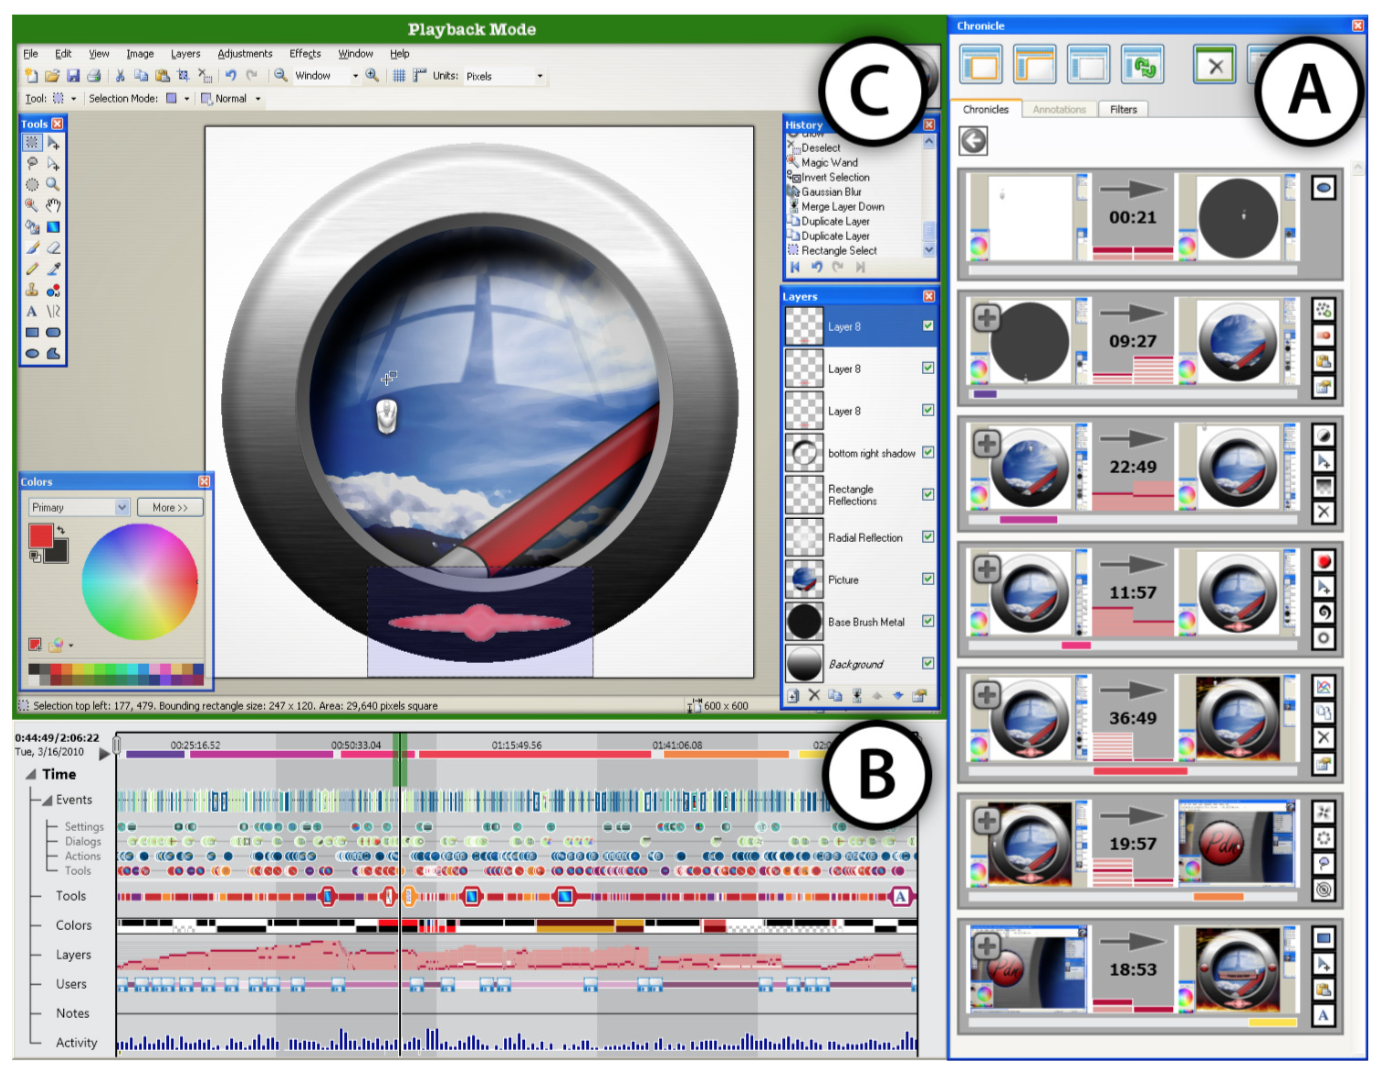
\includegraphics[width=0.4\textwidth]{\background/fig/software_viz/Grossman}
  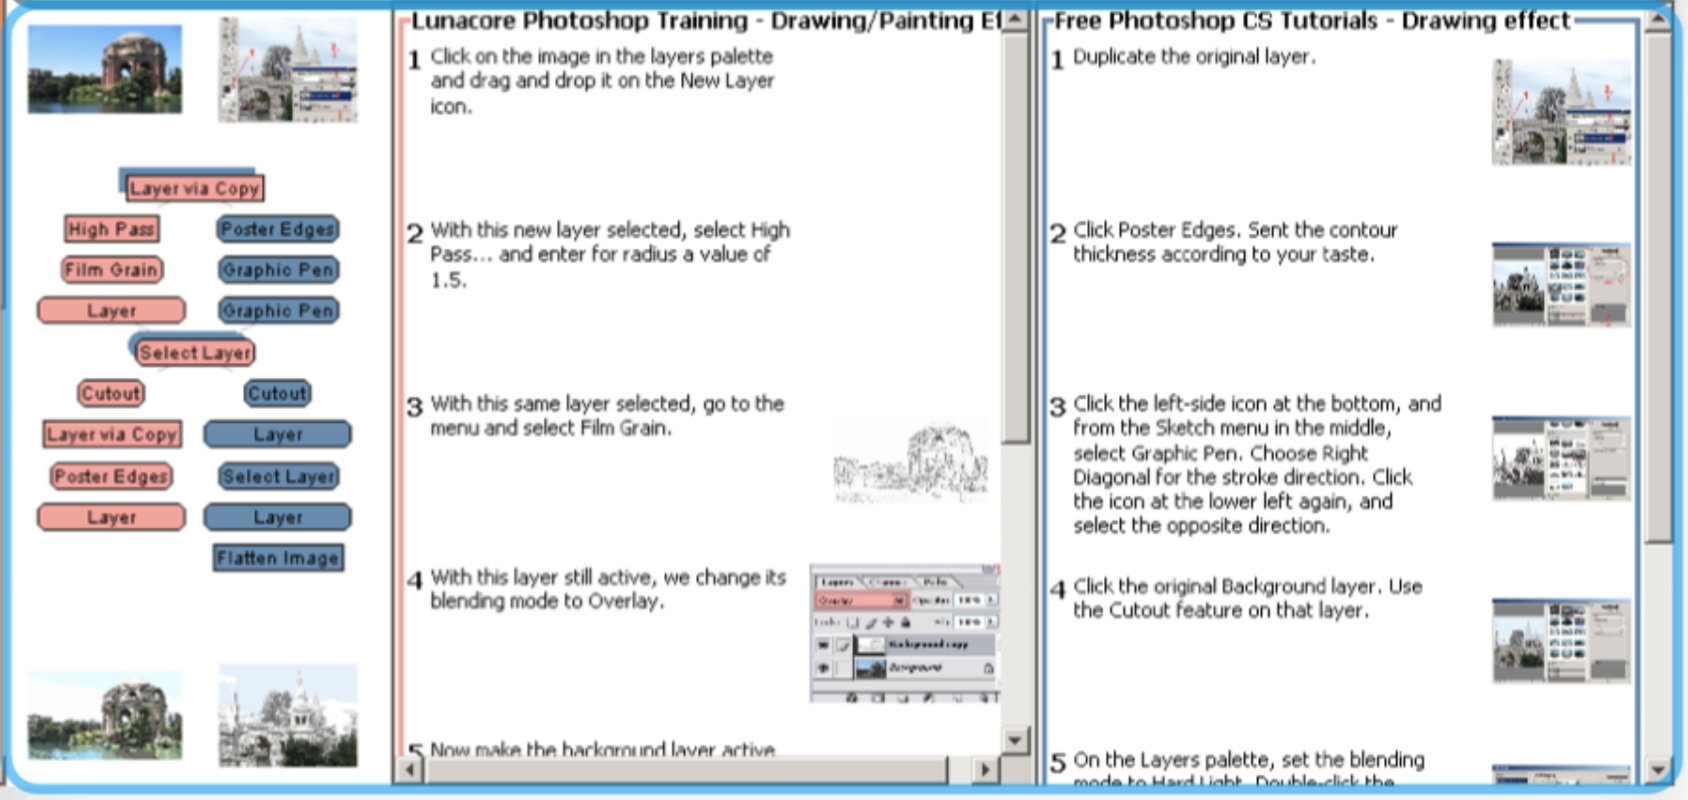
\includegraphics[width=0.55\textwidth]{\background/fig/software_viz/Kong}
  \caption{Instructional systems that help learners compare effects and similar tutorials using (left) before and after images (a) and event timeline (b) by Grossman \ea{}~\cite{Grossman:2010jz} and (right) operation union graph by Kong \ea{}~\cite{Kong:2012:DTR:2207676.2208549}.}
  \label{fig:related_comparison}
\end{figure*}

% summary
These systems provided insights on 1) automatic generation methods of step-by-step tutorials and 2) workflow presentations serving for different purposes. Our MixT system is built based on the Photoshop plug-in (Tutorial Builder) to acquire a step-by-step document with text descriptions. We enhance the static tutorial format by embedding instructional video clips for each operation that can be interactively reviewed.

This paradigm opens a design space to create new tutorial formats that can be interactively reviewed. In recent years, researchers have shown that learners using responsive video tutorials~\cite{Nguyen:2015:MST:2702123.2702209} and learning-by-doing activities~\cite{Kwon:2016:CEO:2858036.2858101} performed better in following instructions than using static or video tutorials.

% -------------------

\subsection{In-Application Support}

The above methods introduce innovative ways for learners to review workflows and instructions. However, reviewing these materials is often separated from operating a software application. Learners might have to switch between the main application they are using and a separate set of instructions, which could introduce a gap of evaluation (\iquote{Am I doing this right as the instructions explain?}) and a gap of execution (\iquote{How do I perform the action that the instructions describe?}).
%
Researchers have proposed another approach to provide ``in-application'' assistance, often in real-time, in a specific application context.

There has been a considerable amount of research devoted to offering interactive help to support learners comprehend the functionalities while operating an application.
%
Crystal~\cite{Myers:2006:AWW:1124772.1124832} enables software users ask questions about ``why'' something did or did not occur in an application.
%
Video snippets can be embedded in application tooltips to explain specific functionalities~\cite{Grossman:2010wr}, which were shown to be seven times more effective than conventional tooltips for completing unfamiliar tasks.

Interactive, step-by-step instructions can be integrated in several forms:
%
To help software users identify specific UI components, tutorials can be shown via a translucent colored ``stencil,'' which visually directs user's attention in an application~\cite{Kelleher:2005:STD:1054972.1055047}.
%
By tracking user's current operations, tutorials can be embedded in an application to provide instant feedback such as a check-mark or a percentage match~\cite{Fernquist:2011:SRE:2047196.2047245}, automatically replayed to present the corresponding video instructions~\cite{Pongnumkul:2011ju}, or be shown as ambient help~\cite{Matejka:2011:AH:1978942.1979349}.
%
Instructions can be captured from demonstration as ``scripts'' for step-by-step navigation~\cite{Bergman:2005:DocWizards}. In-application controls~\cite{Lieberman:2014:SML:2557500.2557543} and game elements~\cite{Li:2014:CGM:2556288.2556954, Dontcheva:2014:CCL:2556288.2557217} can further engage users in learning.

As tutorials are built for a broader community with a set of authors and learners, content can be dynamically updated within a community based on user contribution~\cite{Lafreniere:2013ff,Matejka:2009:CCR:1622176.1622214, Bunt:2014:TPI:2556288.2557118}.

Our work focuses on authoring tools to create novel tutorial format designs, not the learning support. We see opportunities of combining our approaches with in-application guidance. For example, a video clip from a MixT tutorial can be automatically replayed when a system detects a slowdown of a learner's progress on a specific step. However, we do not claim contribution in this direction.

% These projects show how effective instructional representations can assist learners in learning or executing tasks. Our goal is to further study new formats that incorporate advantages of several formats of multimedia, including images, text, and videos, and in turn enhancing the learning experience for a variety of tasks.

% * define ``automatic''
% Note: MixT tutorials are automatically rendered from manual demonstration, not automatically generated.

% To provide real-time assistance, it is important to recognize the user activities during a task performance. Several domains have been widely studied, including software operations, scene recognition, and object tracking in a physical world.

% -------------------------------------------

\section{Instructions for Physical Activities}
\label{related_physical}

The above approaches of tracking a software demonstration open the door to enable interactive tutorials that can respond to user progress. However, understanding user behavior in the physical world, rather than in software, remains challenging.
%
How do technologies track humans and objects in a space to support real-time feedback? What are the available authoring techniques to generate instructions for physical tasks?
%
This section discusses the challenges from four perspectives, including tracking activities, authoring instructions, presenting guidance, and enabling interactive instruction following in a real world.

% -------------------

\subsection{Tracking Physical Activities}
To record activities and provide responsive feedback, a computer system needs to detect user operations and objects in real-time.
%
Computer vision techniques can automatically track specific physical targets shown in a video for interactive applications. These include three major categories:

\begin{itemize}
  \item \textbf{Tracking objects}. Common techniques include:
  1) Track specific \emph{colors} or visual features of pre-defined objects. Examples include tracking a fast-moving Ping-Pong ball for automatic camera control~\cite{Okumura:2011tr} or paper puppets for creating animation~\cite{Barnes:2008:VideoPuppetry}.
  %
  2) Track both \emph{colors and depths} of objects, which could obtain a better understanding of the objects' positions in a 3D world. The information can be useful for activities involved object manipulations, such as block or toy assembly tasks~\cite{Gupta2012DuploTrack,Wu:2016:ARI:2856400.2856416} and 3D puppet control~\cite{held20123d}.
  %
  3) Track \emph{motion-capture markers}. The most common method is to attach reflective markers to an object's surface. This enables accurate, responsive capturing, such as to record an animator's continuous movements~\cite{Dontcheva:2003:LAC:1201775.882285}.
  %
  \item \textbf{Tracking humans}. Targets include \emph{faces} (e.g., to show a close-up of a speaker during video conferencing~\cite{Ranjan:2010}, provide real-time camera control guidance when filming an interview video~\cite{Carter:2010}, and capture facial performances~\cite{Shi:2014:AAH:2661229.2661290,thies2016face}), \emph{hands} (e.g., to enable gestural control~\cite{taylor-siggraph2016} and camera control of a repair task~\cite{Ranjan:2008}), and \emph{user movements} (e.g., to provide augmented information~\cite{Wilson:2012fb,Anderson:2013:YEM:2501988.2502045}).
  %
  Motion-capture markers are often used to accurately track actors in professional filmmaking. However, since markers are visible in a camera view, visual effects (VFX) are necessary to post-process a video recording.
  %
  \item \textbf{A combination of the above}, such as reconstructing a 3D scene of a player throwing a basketball~\cite{dou-siggraph2016}.
\end{itemize}

Some of these vision-based systems require a high-speed camera~\cite{Okumura:2011tr} or a RGB-D camera~\cite{Gupta2012DuploTrack,Wu:2016:ARI:2856400.2856416,held20123d,Wilson:2012fb,Anderson:2013:YEM:2501988.2502045,dou-siggraph2016}, while some require users to wear reflective markers~\cite{Ranjan:2008}.
%
Other non-vision tracking methods rely on sensors attached to an object or human, including GPS sensor~\cite{HexoDrone} and radio frequency wireless signals~\cite{Nguyen:2016:ICR:2935620.2935632}. These are often used for tracking a moving target in a larger space, such as a flying drone.
%
Finally, if video content is difficult to be extracted, crowdsourcing algorithms have been introduced to structure step-by-step videos by online workers~\cite{Kim:2014:CSI:2611222.2556986}.

% summary
The detection mechanisms from these systems inspired us to design interactive systems that can react to authors' activities without requiring users to carry  a sensor. For examples, Kinectograph and DemoDraw track authors' body parts using a Kinect sensor that has been widely available to consumers.
%
However, tracking technique for high-level information, such as the \emph{intent} of a certain action, is yet lacking. Therefore, when automatic activity recognition is difficult, we include authors in a loop to annotate a task. DemoCut provides an annotation interface for describing DIY videos; DemoDraw provides a multi-modal interface to label continuous body movements.

% These methods usually require an expert defining heuristics of space regions or movement classifications ahead of time for the tracking program.

% -------------------

\subsection{Authoring Instructions for Real-World Tasks}

We identified two major approaches to create instructions for physical tasks: model-based and demonstration-based generation.
%
A \emph{model-based} system analyzes the structure of an object or a task and renders instructions.
%
The approaches by Feiner and Seligmann~\cite{feiner:1985:AEA:1299975.1300548,Seligmann:1991:AGI:127719.122732} considered communicative intent and rules of object manipulation to create 3D illustrations. Their automatically-generated results showed that actions such as snapping latches can be effectively expressed by motion arrows and a cutaway view.
%
By analyzing object geometry and other attributes, Agrawala \ea{}'s~\cite{agrawala2003designing} system automatically renders step-by-step assembly instructions, e.g., for furniture and toys (See Figure~\ref{fig:related_models} left).
%
Technical diagrams can also be generated, such as an exploded view that explains mechanical assembly parts~\cite{li2008automated} and motion illustrations that describe how individual parts are operated~\cite{mitra2010illustrating}. Parts are highlighted using colors, often labeled with text; Casual chain sequence of mechanical interaction can be shown as a list of highlighted figures, annotated with motion arrows (See Figure~\ref{fig:related_models} right).
%
Reversely, an existing technical document can be automatically analyzed and transfered into 3D animation by parsing the parts, orientation, and visual annotations~\cite{Mohr:2015:RTD:2702123.2702490}.

\begin{figure*}[t!]
  \centering
  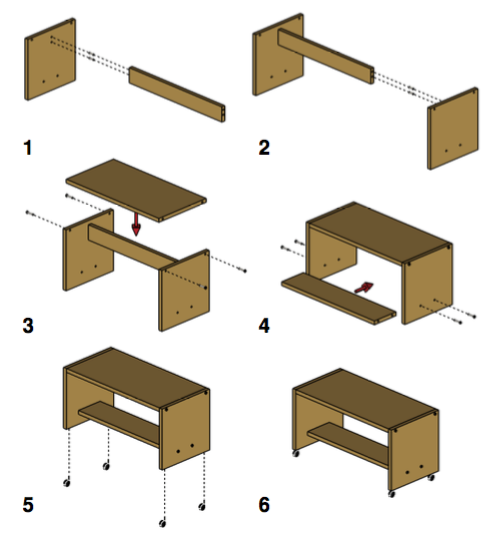
\includegraphics[width=0.3\textwidth]{\background/fig/model_generation/furniture}
  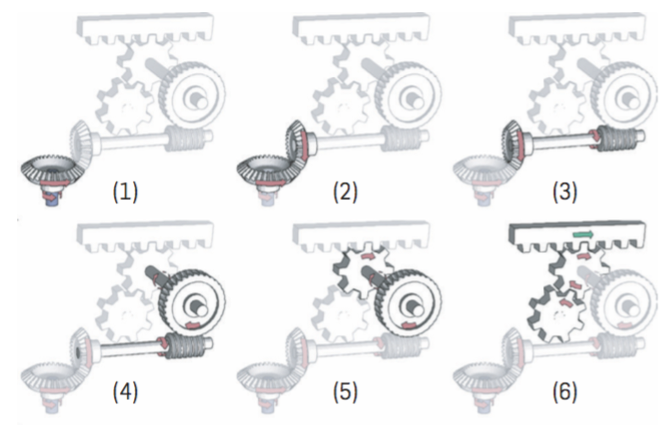
\includegraphics[width=0.5\textwidth]{\background/fig/model_generation/chain}
  \caption{Example instructions automatically generated by Agrawala \ea~\cite{agrawala2003designing} (left) and Mitra \ea~\cite{mitra2010illustrating} (right) using model-based approaches.}
  \label{fig:related_models}
\end{figure*}

A \emph{demonstration-based} system records an author's physical demonstration of a workflow. The captured materials can be either automatically analyzed by the system or manually edited by an author to create instructions.
%
One approach is to employ templates to help users capture sequences of distinct shots (e.g., Snapguide\footnote{\url{http://snapguide.com/}}) or provide a limited set of operations to record specific moments (e.g., adding or removing a part in a block-assembly task~\cite{Ranjan:2007,Gupta2012DuploTrack}).
%
Another approach is to provide an interface to support authors capturing multimedia materials during or after a demonstration, such as using a head-mounted capturing device~\cite{carter2015authoring}. For certain tasks, new recording devices need to be specially designed, such as an integrated device that includes an IR camera to capture a knitting process~\cite{Rosner:2008:SAK:1409635.1409682} and a turntable to record the building process of a DIY project~\cite{Tseng:2015:SPT:2771839.2771869}.

% summary
In this dissertation, we support a wide variety of how-to tasks from craft to home repair and cooking where automatically tracking user activities is not yet completely possible. Since these domains often involve author creativity and personal styles, we opt for the demonstration-based approach.
%
DemoCut, Kinectograph, and DemoWiz each allows authors to perform a physical demonstration in front of a camera, while semi-automatically capturing the activities.

% -------------------

\begin{figure*}[t!]
  \centering
  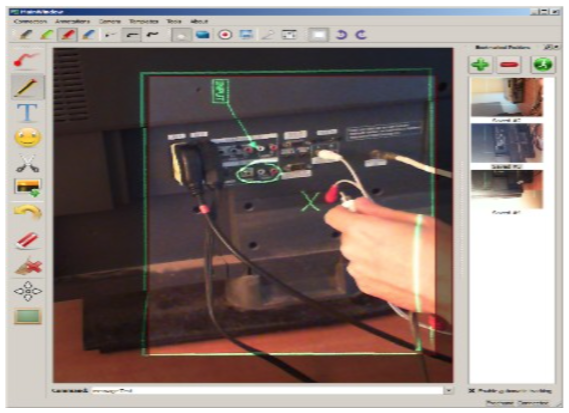
\includegraphics[width=0.4\textwidth]{\background/fig/ar/authoring}
  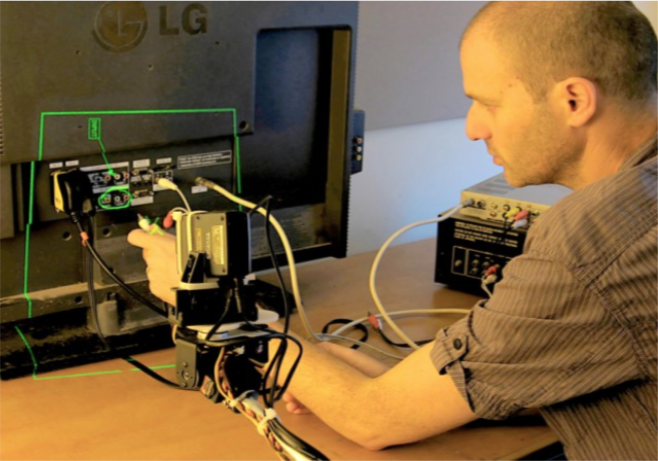
\includegraphics[width=0.41\textwidth]{\background/fig/ar/following}
  \caption{TeleAdvisor~\cite{Gurevich:2012ko} provides an authoring interface (left) for an instructor to guide a remote worker through a repair task (right).}
  \label{fig:related_teleadvisor}
\end{figure*}

\begin{figure*}[t!]
  \centering
  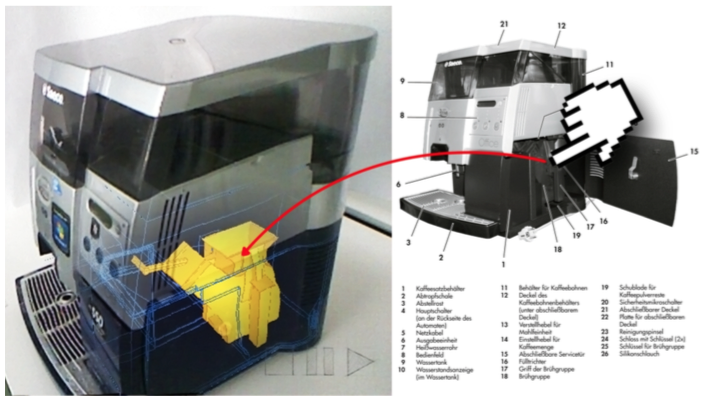
\includegraphics[width=0.55\textwidth]{\background/fig/ar/technical_document}
  \caption{Work by Mohr \ea{}~\cite{Mohr:2015:RTD:2702123.2702490} automatically analyzes a technical document and augments a machine with AR animation in 3D.}
  \label{fig:related_ar_annotation}
\end{figure*}

\subsection{Presenting Guidance}
To help learners perceive instructions for physical tasks, we discuss how guidance can be displayed in a 3D world. There are four main approaches to present real-time guidance.

First, rich information can be shown via an \emph{external display} placed next to the work area. Several applications adopt this method, including cooking~\cite{Uriu:2012:PRM:2207676.2207695} and block assembly tasks~\cite{Gupta2012DuploTrack,Wu:2016:ARI:2856400.2856416}. However, a learner may often switch his or her attention between the task and the instructions. To better blend the information into activities, Knibbe~\ea{} designed a display-embedded table as a physical workspace that monitors, records, and assists users~\cite{Knibbe:2015:SMI:2817721.2817741}. In this way, workers can review the information on the desktop while making a project.

Second, information can be \emph{overlaid on top of the work area} through a projector. Examples include supporting remote repair tasks~\cite{Gurevich:2012ko} (see Figure~\ref{fig:related_teleadvisor} right), assembly tasks~\cite{Kirk:2006:CRG:1124772.1124951}, cooking~\cite{Ju:2001:CIC:634067.634227}, and piano learning~\cite{Xiao:2016:IEI:2858036.2858577}.
%
For tasks such as dance movements, guidance can be shown on an augmented mirror that learners constantly focus on~\cite{Anderson:2013:YEM:2501988.2502045}.
%
This method can effectively present instructions at a location that can be viewed by a learner during a task. However, this often requires a specific indoor environment setup and a calibrated projector, which is not scalable.

Third, information can be \emph{augmented through a head-mounted display or a mobile phone} accessed and viewed by individuals. Researchers have shown AR applications that provide visual highlights for machine maintenance~\cite{Henderson:2011ff,Mohr:2015:RTD:2702123.2702490} (see Figure~\ref{fig:related_ar_annotation}), enable interactive touring in a city~\cite{Feiner1997}, explain product functionalities~\cite{MagicLens}, and present dynamic UI or information based on head orientation~\cite{Zhang:2014:HHO:2659766.2659773}.
%
Compared to the previous approach that projects information onto a public space, this method allows learners to access information individually. Multiple users can interact with an augmented system at the same time. However, learners have to wear or hold a device, which might limit their mobility while performing a task.

Last, for specific tasks, information can be conveyed \emph{directly via target objects}. Haptic feedback has shown to be useful to help learners capture guidance while focusing on the physical tasks, such as for sculpturing~\cite{Zoran:2013:FFD:2470654.2481361,Agrawal:2015:PPS:2807442.2807505}, building multi-material assemblies~\cite{Schoop:2016:DSS:2851581.2892429}, and learning Frisbee~\cite{Solomon:2014:UTI:2540930.2540965}. Visual cues such as LED patterns shown on a device can help direct user's attention~\cite{Solomon:2014:UTI:2540930.2540965,Vasey:2016:HHR:2897839.2927404}.
%
This approach is task-specific and can be difficult to generalize to other task domains.

\subsection{Providing Interactive Guidance}
% \subsubTitleBold{Responding to Learners' Progress}
Finally, we discuss how assistive technologies track a learning process and support interactive guidance. Providing responsive feedback requires an understanding of learners' activities. For specific tasks such as block assembly~\cite{Gupta2012DuploTrack,Wu:2016:ARI:2856400.2856416} and dancing~\cite{Anderson:2013:YEM:2501988.2502045}, learners' progress can be accurately tracked in 3D. This enables a tutorial system to provide real-time information about the current learner state, e.g., where to place the next block to the current model or suggested adjustment on a dance pose.
%
However, as we discuss earlier, tracking activities at the instruction level for real-world tasks is still lacking. Therefore, the majority of the systems provided user interfaces for learners to navigate instructions.
%
For a pair learning scenario, a remote instructor can manually provide instructional input based on the learner's progress that he or she sees, such as highlighting a component for remote repair tasks~\cite{Gurevich:2012ko,Kirk:2006:CRG:1124772.1124951} (see Figure~\ref{fig:related_teleadvisor} left).

Our work focuses on designing tools for tutorial authors to create instructions from demonstrating a task. DemoCut is designed for authoring instructions after the capture time. Kinectograph provides an control interface on a Tablet device for authors to carry and place in a space. DemoDraw's demonstration interface is similar to Anderson \ea{}'s~\cite{Anderson:2013:YEM:2501988.2502045} augmented mirror. But instead of overlaying instructions, we present a real-time rendering view of an author's movements via an external display placed in front of the user. We have not investigated tools for learners to follow a task.

% -------------------------------------------

\section{Working with Videos}
\label{related_videos}

Research in video understanding has introduced new ways to work with videos, including capturing, editing, and navigating. How do authoring tools help users record, organize, and edit necessary materials? What are the interaction techniques of reviewing one or multiple videos? In this section, we review these topics briefly.

% -------------------

\subsection{Capturing}
Tool supports at the capturing phase include:

\subsubTitleBold{Filming Suggestion}
Several research systems guide users at capture time to yield higher-quality videos. Real-time suggestions include framing of the subject or camera view (e.g., NudgeCam for interview videos~\cite{Carter:2010}) and actor's performance~\cite{Heer:2004ba,Davis:2003cu}. Shot suggestions can also be bootstrapped through user dialogs~\cite{Adams:2005}.
%
Patterns from expert storytellers and commonsense reasoning can recommend novice authors to capture materials and develop a story structure~\cite{Barry:2003:MCC:957013.957152,Kim:2015:MSN:2702123.2702507}.

\subsubTitleBold{Camera Control}
Viewpoints of stationary cameras can be automatically decided based on heuristics at record time to trace an actor, an area, or an object~\cite{Ranjan:2008,Okumura:2011tr}.
%
In recent years, quadrotor cameras enable a wide range of trajectories to capture a subject from different viewing angles. Roberts and Hanrahan~\cite{Roberts:2016:GDF:2897824.2925980} proposed an authoring tool for authors to plan and preview a camera trajectory. When being filmed, 3D gestures allow a person to control a quadrotor camera at the scene~\cite{Cauchard:2015:DME:2750858.2805823,Pfeil:2013:EGM:2449396.2449429}.

% summary
We proposed Kinectograph prior to these systems of quadrotor camera control. A recent commercial system has included a similar feature to track a moving user~\cite{HexoDrone}, which is based on GPS location instead of specific body parts.

% -------------------

\subsection{Editing}
Tool supports for video composition and editing include:

\subsubTitleBold{Annotation}
Researchers have investigated how to provide interactions that enable efficient, fluid annotation or labeling of video data. Examples include the EVA system~\cite{Mackay:1989} that encouraged authors to annotate materials at capture time. More recent interfaces leverage pen input (e.g., VideoTater~\cite{Diakopoulos:2006vt}) and touch or gestural input~\cite{Sarkar:2016:SCC:2858036.2858199}.

\subsubTitleBold{Story Composition}
When working with a repository of video clips, it can be challenging to compose a compelling story. Several new interaction techniques have been proposed:
%
A storyline can be created non-linearly based on relevant characters, emotions, and themes of the current edited clips~\cite{Shen:2009:WNE:1518701.1518825}.
%
Tangible controllers with a specialized table interface enable collaborative, non-linear editing~\cite{Bartindale:2012:STS:2207676.2207700,Bartindale:2016:TSS:2818048.2819929}.
%
Live authoring at capture time with a Tablet device allows an author to quickly organize clips and apply editing decisions~\cite{Freeman:2014:LLA:2611105.2557304}.

\subsubTitleBold{Computer-Powered Editing}
Frame-based editing of video is very time-intensive, as it forces users to operate at a very low level of detail. Editors can leverage \emph{metadata}, such as shot boundaries~\cite{Casares:2002dx} and transcripts~\cite{Berthouzoz:2012} that help users place cuts and transitions. This gives users higher-level editing operations at the shot level rather than the frame level.
%
Techniques of \emph{computer vision} and \emph{speech analysis} can automate certain visual effects, such as creating cinemagraphs~\cite{Bai:2012, Joshi:2012}, automatically-edited lecture videos~\cite{Heck:2007}, zoomable tapestries~\cite{Barnes:2010} and synopses~\cite{Pritch:2009vl}, or stabilizing shaky amateur videos~\cite{Liu:2011}.
%
Edits can take place during recording, such as switching to a close-up view of a person who is speaking~\cite{Ranjan:2010}.
%
When material can be reviewed in 3D such as character animation, camera angles can be optimized to render a new video by analyzing the actor data~\cite{assa2005action,assa2008motion}.
%
Finally, when video analysis is a matter of subjective taste, identifying salient frames or highlights can be outsourced to crowd workers~\cite{Bernstein:2011uj,Tang:2012:ECS:2207676.2208622}.

% summary
MixT, DemoCut, Kinectograph, and DemoDraw also use vision techniques for automatic editing. They differ from previous approaches in its focus on two particular application domains -- software and physical demonstration videos.
%
By focusing on a specific domain, MixT and DemoCut can make assumptions about the structure of the input and output video, such as the fact that there is a linear set of steps, and offer an interface and algorithms that make it easier to create high quality how-to videos.
%
Kinectograph makes editing decisions (e.g., pan-and-tilt, zooming) based on actor's body location for instructional videos.
%
DemoDraw includes a multi-modal interface where authors can annotate a motion recording using speech while physically performing movements.

% visual enhancement~\cite{Santosa:2013:DST:2470654.2466148}

% -------------------

\subsection{Navigating}
% Tool supports for video navigation include:
Automatic video control can follow user actions or preferences, such as segment playback when operating software applications~\cite{Pongnumkul:2011ju} or playback speed control~\cite{Cheng:2009:SUV:1518701.1518823}.
%
Videos can be navigated at the content level beyond a linear timeline, such as visualizing subject movements in a storyboard design~\cite{goldman2006schematic} or a continuous image mosaic~\cite{Teodosio:2005:SS:1047936.1047940} and enabling direct manipulation of a target in 2D~\cite{Dragicevic:2008:VBD:1357054.1357096,Goldman:2008:VOA:1449715.1449719,Karrer:2008:DDM:1357054.1357097} or 3D~\cite{Nguyen:2013:DMV:2470654.2466150}.
%
These techniques help viewers understand content flow and playback videos, and have been applied to screencast videos~\cite{Denoue:2013:RDM:2451176.2451190,Nguyen:2015:MST:2702123.2702209}.
%
To further navigate a long video or a set of videos, a canvas showing video tiles and timeline was shown to be 36\% faster than a conventional list view~\cite{Al-Hajri:2014:VPH:2611105.2557106}. A video digest is effective in browsing and skimming video content~\cite{Pavel:2014:VDB:2642918.2647400}.
% Lecture videos~\cite{Tang:2006:DIU:1111449.1111523},

These novel forms of video navigation inspired us to explore new visual and playback designs for revealing the video content.
%
MixT supports per-step video navigation embedded in a static tutorial.
%
DemoWiz augments a screencast video with novel visualization for following the content.
%
DemoDraw renders a series of human movements as concise motion illustrations.

% In contrast to these systems, we do not require the author to manipulate the camera or system during capture. Many leisure activities, such as home repair or cooking, require use of both hands or involve getting one's hands dirty, so camera manipulation is not possible. We use vision techniques for automatic recording and editing. It differs from previous approaches in its focus on particular application domains -- software and physical demonstrations. By focusing on specific domains, we can make assumptions about the structure of the input and output video, such as the fact that there is a linear set of steps or movements, and offer user interfaces and algorithms that make it easier to create high quality instructions.
